\section{Background and Problem Formulation}\label{sec:problem}
%\subsection{Preliminaries}
Consider a robot manipulator capable of grasping and releasing objects in a table-top workspace. 
%
The robot can be tasked with instructions such as ``place the green block on top of the red object and the yellow block on top of the green one" that require the robot to sequentially manipulate objects to achieve an intended block assembly. 
%
We assume that the robot perceives the world through the visual sensor and is equipped with a primitive skill for grasping a specified object and releasing it at a given pose on the table or on another object. 
%
Further, we assume the presence of a planning model, $\mathcal{M}$, which given an initial world state $S_I$ and a goal specified as a language utterance $\mathit{\Lambda}$, can synthesise a plan $\mathbf{\Pi_{S_I}}$ for the robot to execute. 

We build on~\citep{Kalithasan2022LearningNP}, a contemporary neuro-symbolic planner that can learn grounded models for spatial concepts (left, right, on top etc.) as well as actions (e.g, moving and object to a prescribed location)


We consider the problem of detecting and recovering from errors in a table-top setting. The original plan $\mathbf{\Pi_{S_I}}$ comes from an underlying neuro-symbolic planner \cite{Kalithasan2022LearningNP}, $\mathcal{M}$, that takes as input the pair ($S_I$, $\mathit{\Lambda}$). Here $S_I$ is the object-centric representation of the initial state in the form of RGB-D image with bounding boxes and $\mathit{\Lambda}$ is the natural language instruction that guides the object-level manipulation. The planner outputs a sequence of triplets ($a_t$, $o_{1t}$, $o_{2t}$), where $a_t$ is the symbolic action and, $o_{1t}$ and $o_{2t}$ are the indices of the \textit{subject} and \textit{object} of the manipulation task respectively. Figure~\ref{fig:nsrm} shows an input-output example for this neuro-symbolic planner. In addition, the planner has also learnt the effects of the symbolic actions, thus, enabling plan's execution by a robot.

\begin{figure}[h!]
    \begin{subfigure}{1.0\hsize}
         \centering    
         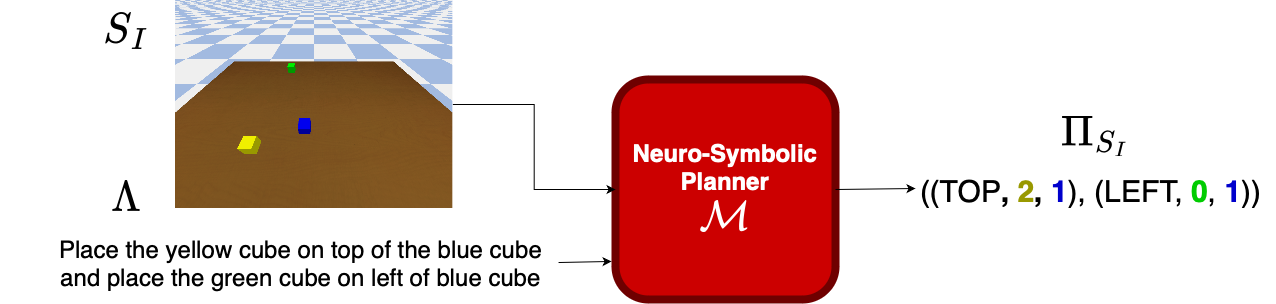
\includegraphics[scale=0.19]{figures/nsrm.png}
    \end{subfigure}
    \caption{
        \footnotesize{
            Sample
        }
    }
    \vspace{-0.15in}
    \label{fig:nsrm}
\end{figure}

%\subsection{Problem}
% To represent the effect of executing a symbolic action $A = (a_t, o_{1t}, o_{2t}) \in \mathcal{A}$ on the state $S \in \mathcal{S}$, we define a function: $\mathcal{E}: \mathcal{S} \times \mathcal{A} \rightarrow \mathcal{S}$. The state $\mathcal{E}(S, A)$ will be reached if the symbolic action is executed by the robot without any disturbances. Similarly, we define $\mathcal{F}: \mathcal{S} \times \mathcal{P} \rightarrow \mathcal{S}$ to denote the state reached after an ideal execution of the input plan on the input state. Formally, for any $S \in \mathcal{S}$ and $\Pi \in \mathcal{P}$, $\mathcal{F}(S, \Pi) = \mathcal{F}(\mathcal{E}(S, \Pi[:1]), \Pi[1:])$.
We represent the effect of executing a plan $\mathbf{\Pi} \in \mathcal{P}$ on the state $S \in \mathcal{S}$ as a function, $\mathcal{E}: \mathcal{S} \times \mathcal{P} \rightarrow \mathcal{S}$. The state $\mathcal{E}(S, \mathbf{\Pi})$ will be reached if the plan is executed by the robot without any disturbances. However, in real situations, the execution may be prone to disturbances, either \textit{internal} or \textit{external}, and may lead the table-top to an \textit{unplanned} intermediate state, $S_E$. The problem then becomes to find a new symbolic plan $\mathbf{\Pi_{S_E}}$, such that $\mathcal{E}(S_E, \mathbf{\Pi_{S_E}}) =_\mathcal{S} \mathcal{E}(S_I, \mathbf{\Pi_{S_I}})$. The relation $=_\mathcal{S}$ on $\mathcal{S}$ holds if and only if the 3D positions of the corresponding objects in the two states are within some $\delta$ threshold. Figure~\ref{fig:rollout} shows the ideal and erroneous execution of the plan generated in Figure~\ref{fig:nsrm}, and how a recovery plan $\mathbf{\Pi_{S_E}}$ is used to repair the original plan $\mathbf{\Pi_{S_I}}$.

\begin{figure}[h!]
    \begin{subfigure}{1.0\hsize}
         \centering    
         \includegraphics[scale=0.19]{figures/rollout.png}
    \end{subfigure}
    \caption{
        \footnotesize{
            Sample
        }
    }
    \vspace{-0.15in}
    \label{fig:rollout}
\end{figure}

Formally, let $\Pi \in \mathcal{P}$ be a sequence of $T$ symbolic actions ($T \geq 1$) and $S \in \mathcal{S}$ be the initial state. Mathematically, $\Pi = (\pi_1, \pi_2, .., \pi_T)$, where $\pi_i \in \mathcal{A}$ are the symbolic actions. We define function, $\mathcal{K}: \mathcal{S} \times \mathcal{A} \rightarrow \mathcal{S}$, to represent the effect of a symbolic action on a state under ideal conditions. Using $\mathcal{K}$, we break-down the function $\mathcal{E}$, thus, capturing its recursive nature. So, for any $T \geq 1$, $S \in \mathcal{S}$ and $\Pi = (\pi_1, \pi_2, .., \pi_T) \in \mathcal{P}$, we have:
\begin{equation}
    \mathcal{E}(S, \Pi) = \mathcal{E}(\mathcal{K}(S, \pi_1), (\pi_2, \pi_3, .., \pi_T))
\end{equation}
Further for each $t \leq T$, we inductively define $S_t = \mathcal{K}(S_{t - 1}, \pi_t)$, where $S_0$ is the initial state. These $S_t$'s represent the \textit{intended} intermediate states for the robot.
% Formally, let $\mathbf{\Pi} \in \mathcal{P}$ be a sequence of $T$ symbolic actions ($T \geq 1$) and $S \in \mathcal{S}$ be the initial state. Define $\mathbf{\Pi_t} := \mathbf{\Pi\left[:t\right]}$, i.e., sequence of first $t$ symbolic actions of $\mathbf{\Pi}$; and $S_t = \mathcal{E}(S, \mathbf{\Pi_t}) \in \mathcal{S}$ for each $t \leq T$. 
In real situations however, the robot may find the intermediate states to be different than the ones expected ($S_t$) due to disturbances. So, let the states encountered during actual execution be $S'_t$, $t \leq T$. Therefore, the problem breaks down into two broad sub-problems: (i) For each $t$, identifying whether $S'_t =_\mathcal{S} S_t$ before executing action $\pi_{t + 1}$, and (ii) If $S'_t \neq_\mathcal{S} S_t$, then finding a plan $\mathbf{\Pi_{E(t)}}$ such that $\mathcal{E}(S'_t, \mathbf{\Pi_{E(t)}}) =_\mathcal{S} S_k$ for some $k \leq T$. Later, we can append the sequence $(\pi_{k + 1}, \pi_{k + 2}, .., \pi_T)$ to $\Pi_{E(t)}$ to get the overall plan $\Pi_{S_t'}$, such that $\mathcal{E}(S_t', \Pi_{S_t'}) =_\mathcal{S} S_T$. 

We seek to learn neuro-symbolic models for $=_\mathcal{S}$ and $\mathcal{K}$ which will help in solving (i) and allowing us to plan in symbolic plan space $\mathcal{P}$, thereby solving (ii) as well. Lastly, in solving (ii), we also seek to find the optimal state $S_k$ to which we can recover in minimum number of steps, thus, making the recovery process faster.